
The proposed autoscaling system scales a web application in response to change in throughput at fixed intervals, which we denote by reconfiguration intervals set to 10 minutes.  This system operates alongside the services deployed by ConPaaS, an open-source runtime environment for hosting applications in Cloud infrastructures~\cite{conpaasIC}. Nevertheless, it can also be easily integrated into any other PaaS, as it only relies on two common services provided by any platform: the resource manager and the monitoring engine. To feed this system, we use the monitoring engine that tracks the application-workload and system resources. Thus, as shown on Figure~\ref{autoScalingSys}, the architecture of our system has the following key components:

%aThis system is able to provision the right amount and type of resources for minimizing the number of SLA violations while keeping the operational cost adapted to the customer requirements.

%Vertical and horizontal scaling actions can be applicable to satisfy the service demand. 


%To choose a scaling plan, provisioning systems have to know the computing capacity of the different server configurations when running an application. To do that, the system creates profiles for each instance type by analyzing its performance behavior (e.g. measuring the cpu usage, request rate and response times). 

\textbf{Profiler:} This component was designed to measure the computing capacity of different hardware configurations when running an application. To do that, this component creates profiles for each resource type (VM instance in the following) by analyzing its performance behavior (e.g. the percentage of CPU usage, request rate and response time).  As we mentioned, the definition of profiles per-instance type improves the accuracy of the scaling actions, specifically in heterogeneous cloud infrastructures. Thus, the \emph{Profiler} component calculates the \emph{optimized throughput} of each type of provisioned configuration. Here an \emph{optimized throughput} is the performance pattern under which a resource assures the QoS requirements while avoiding its under/over-utilization.

% without any server instrumentation.




%However, this operation becomes more problematic by the fact that Web application workloads are often very unstable following an irregular pattern, with occasional short traffic spikes.

\textbf{Predictor:} To prevent SLA violations in advance, workload prediction is needed to estimate the incoming traffic. Inspired by~\cite{wolski_network_1999}, our \emph{Predictor} component takes the monitoring data as input and uses different time-series analysis techniques to predict the future service demand for the next monitoring window. To provide accurate forecasting measures, this component utilizes the technique that exhibited the lowest cumulative error measure during the previous monitoring window. By doing so, the \emph{Predictor} is able to adapt the predictions to the current type of workload. This component supports five distinct statistical models that fits four types of workload: \emph{(1)} \emph{Linear Regression} for linear trends~\cite{muppala_regression-based_2012}, \emph{(2)} \emph{Auto Regression Moving Average} (ARMA) for linear with small oscillations~\cite{roy_efficient_2011}, \emph{(3)} \emph{Exponential Smoothing Holt Winters} for daily and seasonal~\cite{exponential_smoothing2010}, and \emph{(4)} \emph{Autoregression} and \emph{Vector Autoregression} for correlated trends~\cite{chandra_dynamic_2003}. 




\textbf{Dynamic load balancer:} In order to adapt our system to the heterogeneity of requests and cloud resources, this component dynamically adjusts weights to the backend servers to proportionally distribute the incoming traffic based on the performance capacities of each provisioned resource. As an example, a server with four cores is able to process a higher number of requests, thus its weight is usually greater than a server with only one core.


\textbf{Scaler:} This component governs our autoscaling system. As illustrated in Figure~\ref{autoScalingSys}, the \emph{Scaler} uses the \emph{Predictor} and \emph{Profiler} components to find the scaling plan that fulfills a pre-established SLO, and consequently better enforces customer preferences. Furthermore, this component constantly analyzes the behavior of each provisioned VM, triggering the \emph{Dynamic load balancer} component when necessary.

\begin{figure}[t]
  \begin{center}
    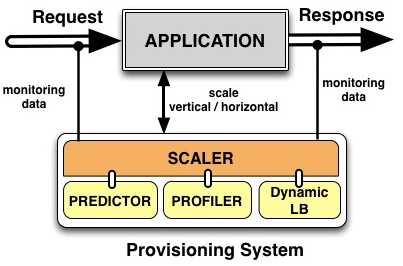
\includegraphics[width=.7\linewidth, height=3cm]{images/monitoringSchema}
  \end{center}
\vspace{-4mm}
  \caption{Autoscaling system.}
  \label{autoScalingSys}
\end{figure}

In the following section, we focus on answering \emph{when} to scale and \emph{which scaling plan} to choose when running web applications. Note that for simplicity, detailed description of the \emph{Predictor} and \emph{Dynamic LB} components are out of the scope of this work.